% !TEX root = CSC104LectureNotes.tex

\setcounter{chapter}{10}
\chapter{Introduction to Python}
\label{day:python1}

\topquote{Talk is cheap. Show me the code.}{Linus Torvalds}

\minitoc

\begin{note}{Read the Textbook}
Now that we have begun the programming phase of the course, it is \textit{very important} that you add reading the textbook to your list of pre-class preparation activities.  From here on out, these notes will highlight the topics to be covered, but the textbook and its associated activities will provide the most complete information and preparation for class.\\

Please note that the textbook is \textit{interactive}.  It is not meant to just be read; you will be clicking on things, and eventually even typing in code, while you work through the chapters.  Frequently, your homework grade will depend at least in part on completing these interactive activities.\\

Programming is similar to many other pursuits in that you will only get better with practice.  The textbook is meant to give you these opportunities.  Make sure to take advantage of them.
\end{note}

\section{An Example Program}

Let's look at what Python source code looks like.  Here's a simple program to get you started.

\begin{py}{Hello World}{hw}
print("Hello world!")
\end{py}

It is a tradition in Computer Science, when learning a new programming language for the first time, to learn how to write a program that displays the message ``Hello world!'' to the screen.  The Code Listing you see above in Listing \ref{lst:hw} does just that.

Many people are surprised to learn that we can write a functional Python program in just one line of code, but that's exactly what we have here.  Python was designed to be simple to learn, and simple to use.

\section{How to Write and Run the Hello World Program}

Python is not only a simple programming language to learn, it also comes with some very easy-to-use tools for programming.

There is no shortage of Python programming environments that we can download and use.  Some are \textit{open source}\footnote{Stuff about FOSS}, and some are commercial.  Some are very simple to get started with, but provide somewhat limited functionality for professionals; and others have lots of features but may be too complicated for the first-time programmer.  In this course, we will be using one of the simple ones.

Appendix \ref{chapter:idle}, which starts on Page \pageref{chapter:idle}, details how to install \addindex{IDLE}{IDLE}, the development environment we will be using this semester.  Once IDLE is running, we can type our program into the interactive Python interpreter, as seen in Figure \ref{fig:idlelinux-hw} on Page \pageref{fig:idlelinux-hw}.

\begin{myfigure}[label=fig:idlelinux-hw]{The Hello World Program in IDLE on Linux}
    \centering
    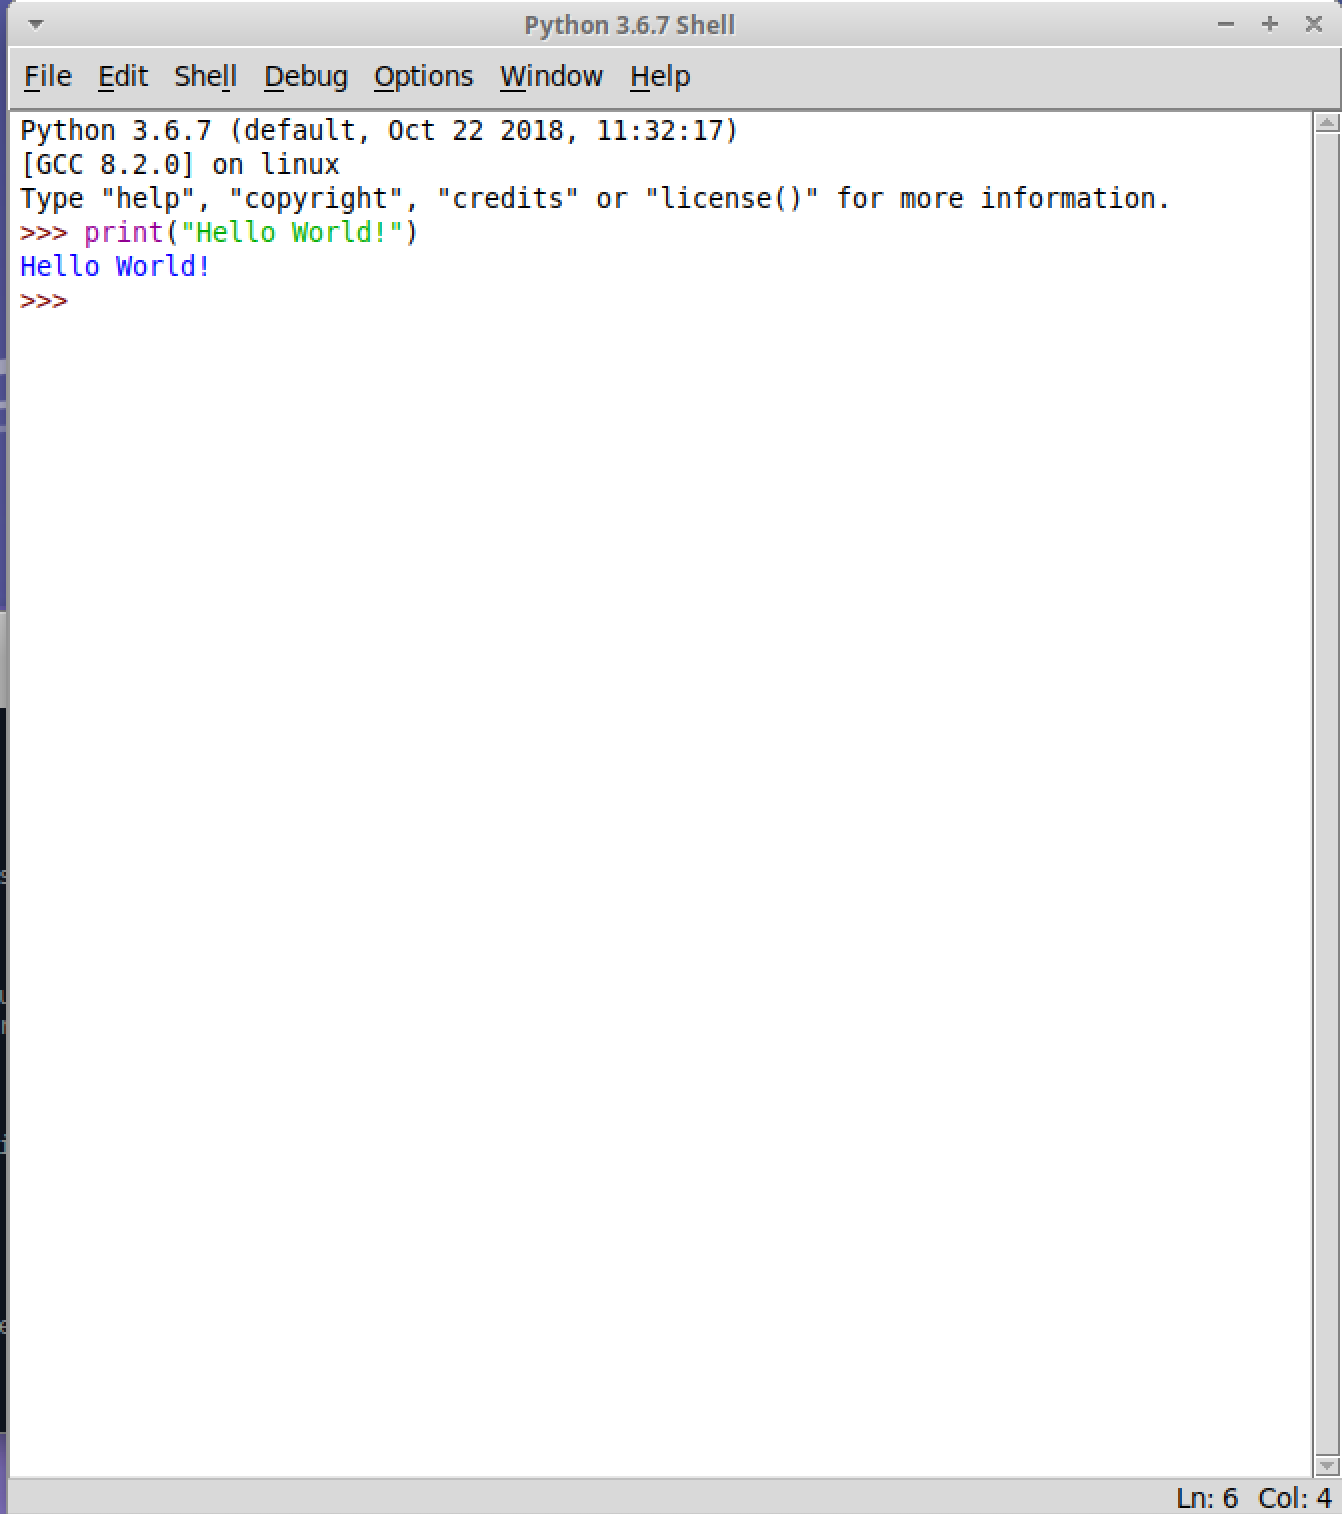
\includegraphics[scale=0.6]{screenshots/idlelinux-hw.png}
\end{myfigure}

In class today, you will start up IDLE for the first time, and type some commands in.

\section{Starting to Program in Python}

As you've read in Chapter 1 of the textbook, most computer programs perform three basic kinds of instructions:

\bi
    \item Input
    \item Processing
    \item Output
\ei

Your instructor will guide you through some examples of each in class.